This chapter will cover the design phase of the project, and the decisions  that were made during. The design phase was integral to the success of the project, requiring a solid design concept to build the application upon.

\section{Initial Idea}
During the initial project meeting an initial project plan was made \ref{appendix:initIdea}, the initial idea proposed the creation of a mobile application using React Native \cite{reactnative} to create the user interface and application logic, and, Firebase \cite{firebase} to store the application data, and, authentication information. The idea was to allow users to create an account, have multiple groups which will have preset and custom locations for users to show their status. Users would have a profile picture that would be used on their clock hand to add to the personalised experience. This application would be used to help groups of friends communicate their status to alleviate the struggles of planning interactions. This initial idea was the starting inspiration for the creation of the application designs, and, the process of eliciting requirements.

\section{Design Decisions}\label{designDecis}
To design and implement this application idea many design decisions and considerations had to made in order to deliver a suitable final product. Although the initial idea proposed the use of React Native and Firebase, other technologies were researched and compared through a comparative study \cite{compStudy} to ensure this was the correct decision. Firebase is a backend-as-a-service, this was chosen over other alternatives due to the ability to create high quality applications in a short amount of time due to the various tools and services Firebase offers. Firebase eliminated security concerns for the storing of data and authenticating of users by handling this internally using Googles security solutions, making Firebase very secure. The decision to create a cross-platform application was made at the initial stages due to the time constraints present in this project. Although native applications can often be more resource efficient and responsive due to being purpose built for a specific operating system, research confirmed that cross platform development can still produce high quality applications. The extra benefits incurred from native development were also not to be exploited in this project, so this was a logical decision, given this research, and, the project time constraints.

\section{Software Architecture}
Model View Controller (MVC) \cite{mvc} is a software architecture pattern that is commonly used in mobile and web application development. This pattern involves a model that contains the data for the application, the view that displays this data to the user, and, the controller which handles interactions between the two. For this project however, the decision was made to use React Native (see \ref{reactSection}) and Firebase (see \ref{firebaseSection}), which has not as clear a distinction between our model, view, and, controller. Firebase is clearly our model storing the application data, and we are using React Native to present our data as the view, but, there is no clear answer as to what is our distinct controller. In this project there is more of a view-controller with our screens interacting with the Firebase database, then rendering our components. An initial component diagram was drawn up to visualise this concept shown in \ref{fig:compDiag}.
\begin{figure}[!htbp]
    \centering
    \begin{subfigure}[b]{0.6\textwidth}
        \frame{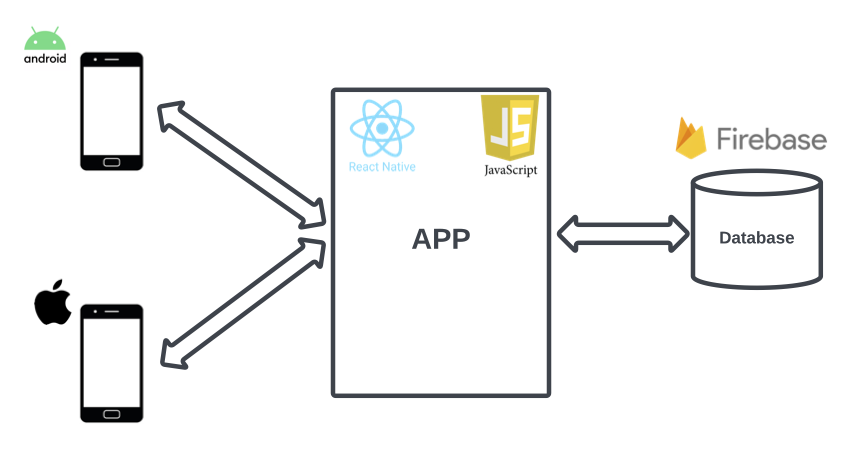
\includegraphics[width=\textwidth]{init-comp-diag.png}}
    \end{subfigure}
    \caption{Initial component diagram of architecture} 
    \label{fig:compDiag}
\end{figure}
\FloatBarrier
Here, we can see that the application code is interacting with Firebase, and then formatting this data to be displayed to the user. The application code is also handling inputs from the user, then preparing this data to then be sent to Firebase. This is still fundamentally a model view controller architecture with separations between storing the data, interacting with the data model, and, displaying the data, but, with the controlling and displaying of data more integrated into a view-controller.

\section{Data \& Media Storage}\label{dataMedStor}
Whilst the database design would likely change throughout the project due to changing requirements and feature development, an initial plan of what data we would need to store, and how, was created. After some initial research it was discovered that Firebase's realtime database does not allow the storage of media, so, their cloud storage would have to be used for media storage, with a path to the image stored in the database. The images required to be stored were the user profile pictures, and, the clock face images. Their were two main categories of data that would need to be stored, users, and, groups.

\begin{figure}[!htbp]
    \centering
    \begin{subfigure}[b]{0.6\textwidth}
        \frame{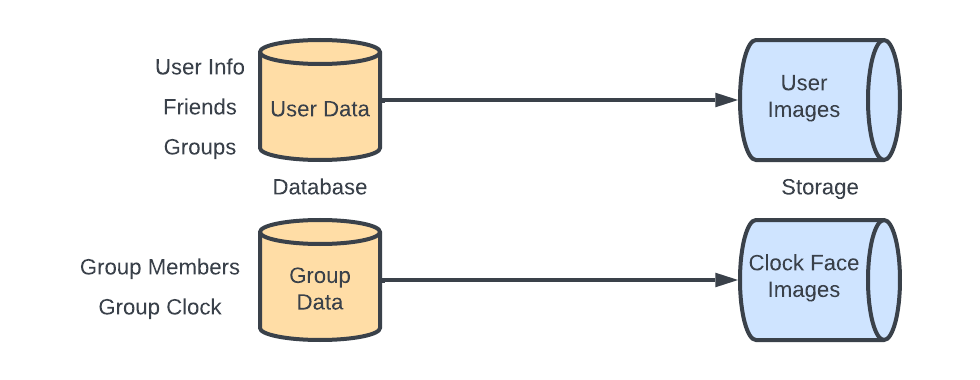
\includegraphics[width=\textwidth]{dataDesign.png}}
    \end{subfigure}
    \caption{Initial data storage design} 
    \label{fig:dataDesign}
\end{figure}
\FloatBarrier

Above is a simplistic representation of the data and media that was required to be stored.
In practice however, these data categories would need to be further separated as nesting sizeable data inside JSON objects can create performance issues. This is apparent when fetching data as all the data inside the JSON object is downloaded, even if the data is not to be used \cite{fbStructData}.

\section{User Interface}\label{UIDesign}
\subsection*{Figma}
To design the user interface some initial sketches were drawn up and then converted into more concrete wire frames. Figma \cite{figma}, an interactive interface design tool was used to create these wire frames. Figma allows the user to create high quality user interface designs that can incorporate animation, leading to the creation of initial design prototypes. Through their mobile application you can visualise these design prototypes on your personal device, enhancing the developer experience and leading to better designs. Shown below are some initial designs that were created through Figma, then later developed into the final application. For the full set of designs see \ref{appendix:figmaScreens}.

\begin{figure}[!htbp]
    \centering
    \begin{subfigure}[b]{0.25\textwidth}
        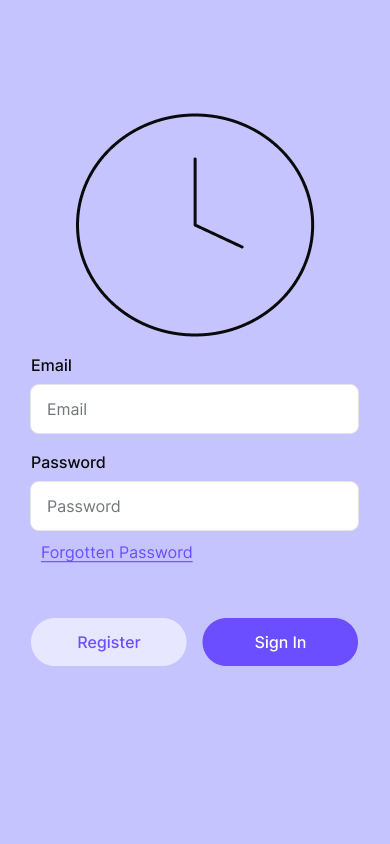
\includegraphics[width=\textwidth]{designSignIN.png}
        \caption{Sign In page}
    \end{subfigure}
    \hspace{1.5em}
    \begin{subfigure}[b]{0.25\textwidth}
        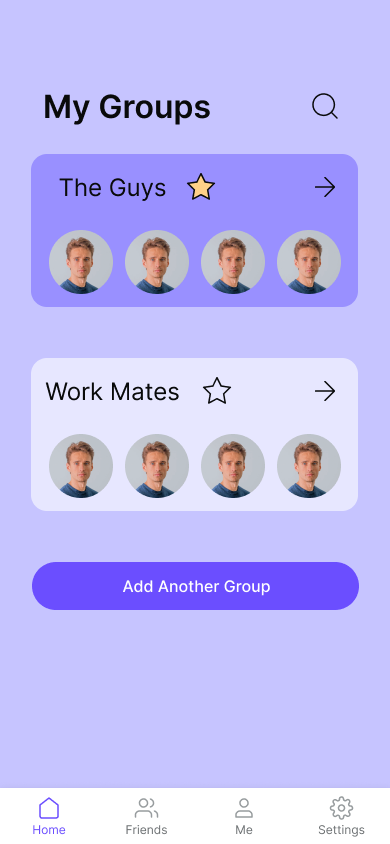
\includegraphics[width=\textwidth]{designHome.png}
        \caption{Home Page}
    \end{subfigure}
    \hspace{1.5em}
    \begin{subfigure}[b]{0.25\textwidth}
        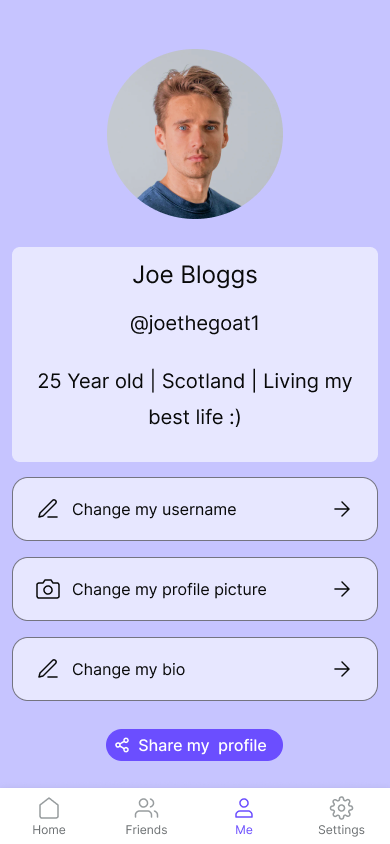
\includegraphics[width=\textwidth]{designProfile.png}
        \caption{Profile Page}
    \end{subfigure}
    \caption{Some initial screen designs from Figma}
    \label{fig:figma}
\end{figure}
\FloatBarrier

\subsection*{Design Motivations}
An aesthetically pleasing and highly accessible application was a must have requirement for this project as listed in \ref{functional}. A high level of detail would have to be put into the initial designs to not only satisfy this requirement, but aid implementation. Rounded corners were used throughout the application instead of sharp edges not only for aesthetics, but this has been said to reduce the cognitive load of users \cite{roundedCorners}, so this was an important concern. The colour scheme of eye catching light and dark purples is used throughout the design, with purple said to spark creativity, and calm users \cite{purplePsych}. Overwhelming the user was also a key concern with a focus on only displaying necessary information so that the visual real estate is being used effectively. The ability for users to personalize their experience is vital to driving user engagement \cite{customUserEng}, so enabling users to upload a profile picture that can be shown in their groups, on the home page, and even on their profile alongside other personalization is vitally important to enhancing the user experience thus driving user engagement. 

\subsection*{App Structure}
The order in which screens are presented, and, navigated is important with respect to the user experience. Users should be able to easily navigate the application with screens presented in a logical, and meaningful order. The app should initially load with a minimalist splash screen (\ref{splash}), then redirect to a sign in screen once the application is loaded. When logged in the users are presented with a home screen including a bottom navigation bar to the three other main pages, friends, my profile, and, settings. This was the basic app structure that was designed, with other relevant pages navigated to from these four main pages. A flowchart displaying the initial desired application flow, and, navigation layout is shown below. 

\begin{figure}[!htbp]
    \centering
    \begin{subfigure}[b]{0.6\textwidth}
        \frame{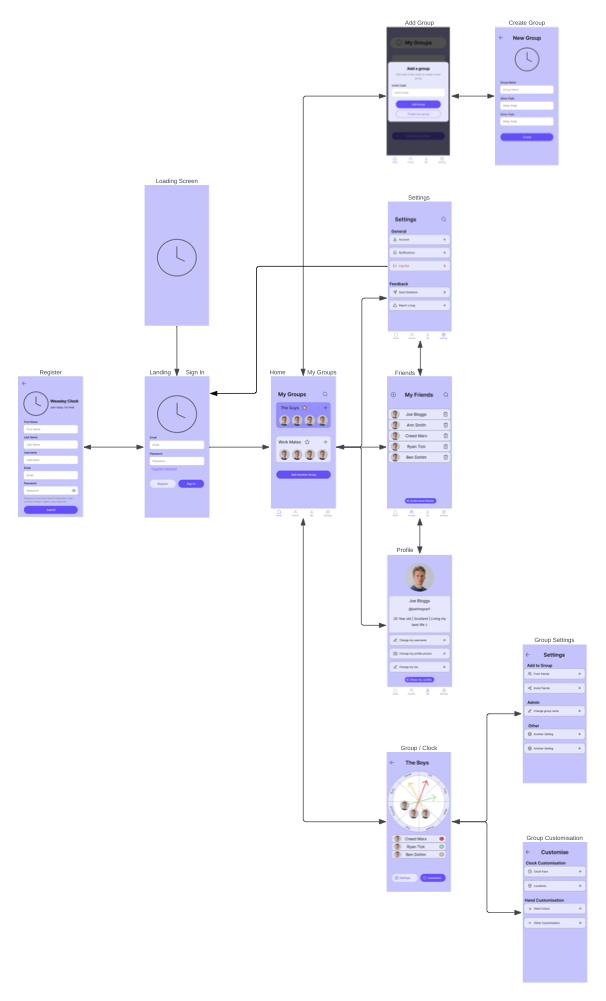
\includegraphics[width=\textwidth]{init-app-pages-flowchart.png}}
    \end{subfigure}
    \caption{Initial desired application, and, navigation layout flowchart} 
    \label{fig:layoutFlow}
\end{figure}
\FloatBarrier

\section{Summary}

In summary, this chapter discussed the design phase of this project, and the decisions made during. An initial idea was created for a mobile application built with a React Native front, and Firebase back. Some initial features that the application would possess were also researched, creating an initial plan for the design of the application. A comparative study was performed on similar technologies to ensure that the choices of technology were optimal for this project. The software architecture, data and media storage, and user interface were all designed to streamline the implementation phase with a robust plan.